\documentclass[aspectratio=169]{beamer}
%[handout]

\usetheme[progressbar=frametitle]{metropolis}
\usepackage{appendixnumberbeamer}

\usepackage[utf8]{inputenc}
\usepackage[T1]{fontenc}

\usepackage[brazil]{babel}
\usepackage[outputdir=..]{minted}
\usepackage{xcolor}
\usepackage{soul} % strikethrough
\usepackage{advdate}
\usepackage{graphicx}
\graphicspath{{figs/}}
\usepackage{graphbox}

\usepackage[ampersand]{easylist}

\usepackage{multirow}
\usepackage{multicol}
\usepackage{subcaption}

\usepackage{pgf,tikz}
\usetikzlibrary{shapes,arrows,positioning}
\usetikzlibrary{circuits.logic.US}
\usetikzlibrary{matrix,calc}

\usepackage{karnaugh-map}

\usepackage{pgfpages}
\setbeameroption{hide notes} % Only slides
% \setbeameroption{show only notes} % Only notes
% \setbeameroption{show notes on second screen=right} % Both

% \graphicspath{{../figs/}}

\definecolor{bgc}{rgb}{0.95,0.9,0.95}
\definecolor{links}{HTML}{2A7F7F}
\hypersetup{colorlinks,linkcolor=,urlcolor=links}

\newminted{verilog}{fontsize=\scriptsize, 
    linenos,
    numbersep=8pt,
    bgcolor=bgc,
    tabsize=4,
    framesep=3mm} 
    %frame=lines,

\newcommand{\verilog}[1]{\verilogf{#1}{\footnotesize}}

\newcommand{\verilogf}[2]{\inputminted[fontsize=#2, 
    linenos,
    tabsize=2,
    numbersep=4pt,
    bgcolor=bgc,
    framesep=3mm]{verilog}{../codes/#1.v}
}

\newminted{nasm}{fontsize=\scriptsize, 
		   linenos,
		   numbersep=8pt,
           bgcolor=bgc,
		   framesep=3mm} 

\usepackage{booktabs}
\usepackage[scale=2]{ccicons}

\usepackage{pgfplots}
\usepgfplotslibrary{dateplot}

\usepackage{hyperref}


\usepackage{xspace}
\newcommand{\themename}{\textbf{\textsc{metropolis}}\xspace}



\usepackage{pifont}% http://ctan.org/pkg/pifont
\newcommand{\cmark}{\ding{51}}%
\newcommand{\xmark}{\ding{55}}%

% \tiny	
% \scriptsize
% \footnotesize
% \small	
% \normalsize	
% \large	
% \Large	
% \LARGE	
% \huge	
% \Huge	



\newminted{python}{fontsize=\scriptsize, 
		   linenos,
		   breaklines,
		   numbersep=8pt,
           tabsize=2,
		   framesep=3mm} 
		   
\newminted{verilog}{fontsize=\scriptsize, 
		   linenos,
		   breaklines,
		   numbersep=8pt,
           tabsize=2,
		   framesep=3mm} 
		   




\definecolor{bgc}{rgb}{0.95,0.9,0.95}
\definecolor{links}{HTML}{2A7F7F}
\hypersetup{colorlinks,linkcolor=,urlcolor=links}


% \usepackage[style=apa]{biblatex}
% \addbibresource{mm.bib}


% \author{\large Prof. Ricardo Menotti (\href{mailto:menotti@ufscar.br}{menotti@ufscar.br})}

\newcommand{\newauthor}[2]{
  \parbox{0.50\textwidth}{
    \texorpdfstring
      {
        \centering
        \small #1 \newline
        {\scriptsize{\urlstyle{same}\href{mailto:#2}{#2}\urlstyle{tt}}}
      }
      {#1} \newline
  }
}

\author{
  \newauthor{Prof. Ricardo Menotti}{menotti@ufscar.br}
\and \newauthor{Prof. Luciano de Oliveira Neris}{lneris@ufscar.br}  
%\and \newauthor{Prof. Artino Quintino da Silva Filho}{artino@ufscar.br}
% \and \newauthor{Prof. Maurício Figueiredo}{mauricio@ufscar.br}
% \and \newauthor{Prof. Edilson Kato}{kato@ufscar.br}
% \and \newauthor{Prof. Roberto Inoue}{rsinoue@ufscar.br}
}

\date{Atualizado em: \today}

\institute{\large \textbf{Departamento de Computação} \\
Centro de Ciências Exatas e de Tecnologia \\
Universidade Federal de São Carlos}

\title{Lógica Digital (1001351)}

\titlegraphic{\hfill
\includegraphics[height=1.5cm]{LogoUfscar}}



\subtitle{Representação Digital da Informação} % 

\begin{document}

\begin{frame}
	\titlepage
\end{frame} 

% \begin{frame}{Conteúdo}
% 	\tableofcontents
% \end{frame}

\section{Representação Digital da Informação} %%%%%%%

\begin{frame}{\insertsection} 
	\begin{itemize}
		\item Nos circuitos lógicos a informação é representada como sinais eletrônicos;
		\item Pode-se considerar que cada sinal representa um dígito de informação; 
		\item Para tornar o projeto de circuitos lógicos mais fácil e preciso, cada dígito pode assumir apenas dois estados:
		\begin{itemize}
		    \item 0 (zero) ou 1 (um);
		    \item L (low) ou H (high);
		    \item F (false) ou T (true);
		\end{itemize}
    \end{itemize}
\end{frame}

\begin{frame}{\insertsection} 
	\begin{itemize}
		\item Esses valores lógicos são implementados como níveis de tensão em um circuito: 
		\begin{itemize}
		    \item o valor 0 é geralmente representado como 0 V (terra);
		    \item o valor 1 é a tensão nível da fonte de alimentação do circuito (normalmente entre 1 e 5 V CC).
		\end{itemize}
		\item Em geral, todas as informações nos circuitos lógicos são representadas como combinações de 0s e 1s;
		\item Antes de iniciar a discussão de circuitos lógicos, será útil examinar como números, dados alfanuméricos (texto) e outras informações podem ser representados usando os dígitos 0 e 1.
    \end{itemize}
\end{frame}

\section{Números Decimais}

\begin{frame}{\insertsection}
	\begin{itemize}
        \item No sistema decimal, um número consiste em dígitos que têm 10 valores possíveis, de 0 a 9, e cada dígito representa um múltiplo de uma potência de 10.
        \begin{itemize}
            \item Por exemplo, o número $8547$ representa $8 \times 10^3 + 5 \times 10^2 +4 \times 10^1 + 7 \times 10^0$
            \item Normalmente não escrevemos as potências de $10$, pois estão implícitas nas posições.
            \item Isso é chamado de representação numérica posicional. 
        \end{itemize} 
        \item Formalmente:
        \begin{itemize}
            \item $D = d_{n-1}d_{n-2} ... d_1 d_0$
            \item $V(D) = d_{n-1} \times 10^{n-1} + d_{n-2} \times 10^{n-2} ... d_1 \times 10^1 + d_0 \times 10^0$
        \end{itemize}
        \item Como os dígitos têm 10 valores possíveis e cada dígito é podendera como uma potência de 10, dizemos que os números decimais são números de base-10.
    \end{itemize}
\end{frame}

\section{Números Binários}

\begin{frame}{\insertsection}
	\begin{itemize}
        \item Como os circuitos digitais representam informações usando somente os valores 0 e 1, não é prático ter dígitos que possam assumir dez valores;
        \item Nesses circuitos, é mais apropriado usar o sistema binário, ou base-2, que possui apenas os dígitos 0 e 1. 
        \item Cada dígito binário é chamado de bit. 
        \item No sistema numérico binário, a mesma representação numérica posicional é usada:
        \begin{itemize}
            \item $B = b_{n-1}b_{n-2} ... b_1 b_0$
            \item $V(B) = b_{n-1} \times 2^{n-1} + b_{n-2} \times 2^{n-2} ... b_1 \times 2^1 + b_0 \times 2^0$
            \item $= \sum\limits_{i=0}^{n-1} b_i \times 2^i$
        \end{itemize}
    \end{itemize}
\end{frame}


\begin{frame}{\insertsection}
	\begin{itemize}
        \item Por exemplo, o número binário 1101 representa o valor
        \begin{itemize}
            \item $V = \textbf{1} \times 2^3 + \textbf{1} \times 2^2 + \textbf{0} \times 2^1 + \textbf{1} \times 2^0$
        \end{itemize}
        \item Como um determinado padrão de dígitos tem significados diferentes para bases diferentes, indicaremos a base como um subscrito quando houver potencial para confusão. 
        \item Assim, para especificar que 1101 é um número de base 2, escreveremos $(1101)_2$. 
        \item Avaliar a expressão anterior para V fornece:
        \begin{itemize}
            \item $V = 8 + 4 + 0 + 1 = 13$
        \end{itemize}
        \item Consequentemente:
        \begin{itemize}
            \item $(1101)_2 = (13)_{10}$
        \end{itemize}
    \end{itemize}
\end{frame}



\begin{frame}{\insertsection}
	\begin{itemize}
        \item O intervalo de inteiros que pode ser representado por um número binário depende do número de bits usados: 
    \end{itemize} 
    \vspace{1cm}
    \begin{table}[]
        \centering \scriptsize 
        \begin{tabular}{cc|cc}
            \hline
             \textbf{Representação} & \textbf{Representação} & \textbf{Representação} & \textbf{Representação} \\
             \textbf{Decimal} & \textbf{Binária} & \textbf{Decimal} & \textbf{Binária} \\
            \hline
            \hline
             00 & 0000 & 08 & 1000 \\
             01 & 0001 & 09 & 1001 \\
             02 & 0010 & 10 & 1010 \\
             03 & 0011 & 11 & 1011 \\
             04 & 0100 & 12 & 1100 \\
             05 & 0101 & 13 & 1101 \\
             06 & 0110 & 14 & 1110 \\
             07 & 0111 & 15 & 1111 \\
            \hline
        \end{tabular}
    \end{table}
\end{frame}


\begin{frame}{\insertsection}
	\begin{itemize}
        \item Um exemplo de um número maior é $(10110111)_2 = (183)_{10}$; 
        \item Em geral, o uso de $n$ bits permite a representação de inteiros positivos no intervalo de $0$ a $2^n-1$;
        \item Em um número binário, o bit mais à direita é geralmente referido como o \textbf{bit menos significativo} (LSB\footnote{\textit{least significant bit}}); 
        \item O bit mais à esquerda, que possui a maior potência de 2 associada a ele, é chamado de \textbf{bit mais significativo} (MSB\footnote{\textit{most significant bit}}). 
        \item Em sistemas digitais, muitas vezes é conveniente considerar vários bits juntos como um grupo:
        \begin{itemize}
            \item Um grupo de \textbf{quatro bits} é chamado de \textit{nibble};
            \item Um grupo de \textbf{oito bits} é chamado de \textit{byte}.
        \end{itemize}
    \end{itemize}
\end{frame}


\section{Conversão entre os sistemas decimal e binário}

\begin{frame}{\insertsection}
	\begin{itemize}
        \item Um número binário é convertido em um número decimal simplesmente aplicando a equação a seguir:
        \begin{itemize}
            \item $V = b_{n-1} \times 2^{n-1} + b_{n-2} \times 2^{n-2} ... b_1 \times 2^1 + b_0 \times 2^0$
        \end{itemize}
        \item Converter um número decimal em um número binário não é tão simples, porque precisamos construir o número usando potências de 2. 
        \item Por exemplo, o número $(17)_{10}$ é $2^4 + 2^0 = (10001)_2$ e o número $(50)_{10}$ é $2^5 + 2^4 + 2^1 = (110010)_2$. Em geral, a conversão pode ser realizada dividindo sucessivamente o número decimal por 2.
    \end{itemize}
\end{frame}

\begin{frame}{\insertsection}
	\begin{itemize}
        \item Converter $(857)_{10}$: 
    \end{itemize}
    \vspace{-0.5cm}
    \begin{table}[]
        \centering \scriptsize 
        \begin{tabular}{rlcc}
              &  & \textbf{Resto}\\
            857 ÷ 2 = & 428 & 1 & LSB\\
            428 ÷ 2 = & 214 & 0 & \\
            214 ÷ 2 = & 107 & 0 & \\
            107 ÷ 2 = & 53  & 1 & \\
             53 ÷ 2 = & 26  & 1 & \\
             26 ÷ 2 = & 13  & 0 & \\
             13 ÷ 2 = & 6   & 1 & \\
              6 ÷ 2 = & 3   & 0 & \\
              3 ÷ 2 = & 1   & 1 & \\
              1 ÷ 2 = & 0   & 1 & MSB\\
        \end{tabular}
    \end{table}
    \begin{itemize}
        \item Resultado  $(1101011001)_2$
        \begin{itemize}
            \item Note que o LSB é gerado primeiro e o MSB é gerado por último;
        \end{itemize}
        \item Estamos considerando apenas a representação de inteiros positivos, depois veremos outras e suas operações aritméticas. 
    \end{itemize}
\end{frame}

\section{Tabela ASCII de caracteres}

\begin{frame}{\insertsection}
    \begin{itemize}
        \item As informações alfanuméricas, como letras e números digitados em um teclado de computador, são representadas como códigos de 0 e 1 dígitos;
        \item O código mais comum usado para esse tipo de informação é conhecido como o código ASCII\footnote{\textit{American Standard Code for Information Interchange}}.
    \end{itemize}
\end{frame}

\begin{frame}{\insertsection}
    \centering
    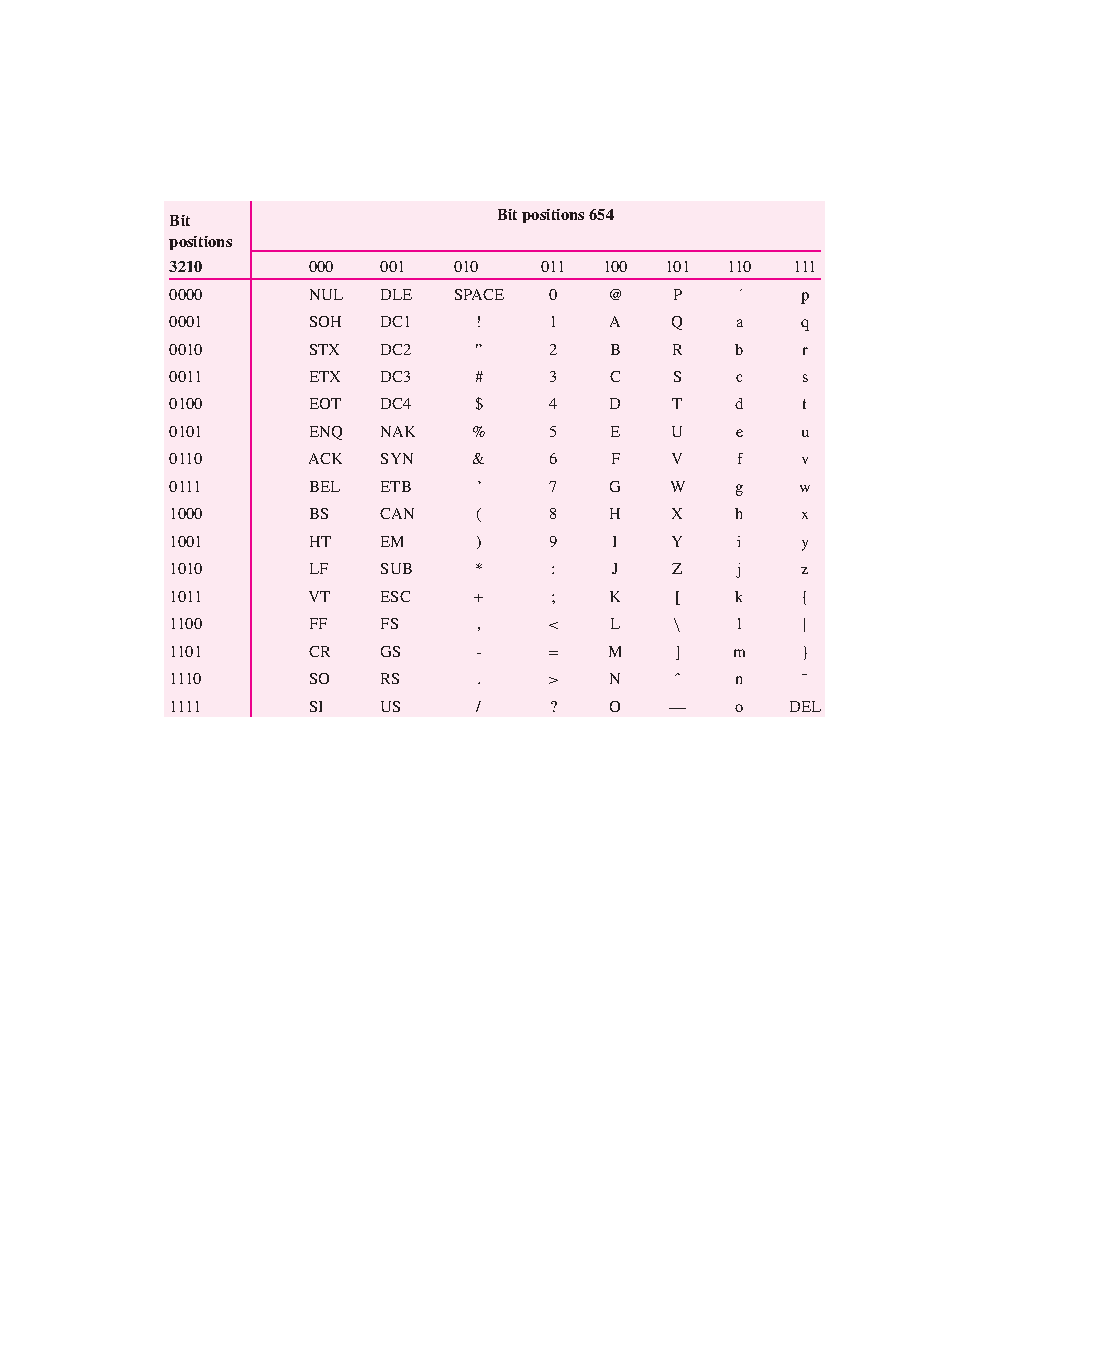
\includegraphics[width=.7\textwidth]{ASCII7} 
\end{frame}

\begin{frame}{\insertsection}
    \centering
    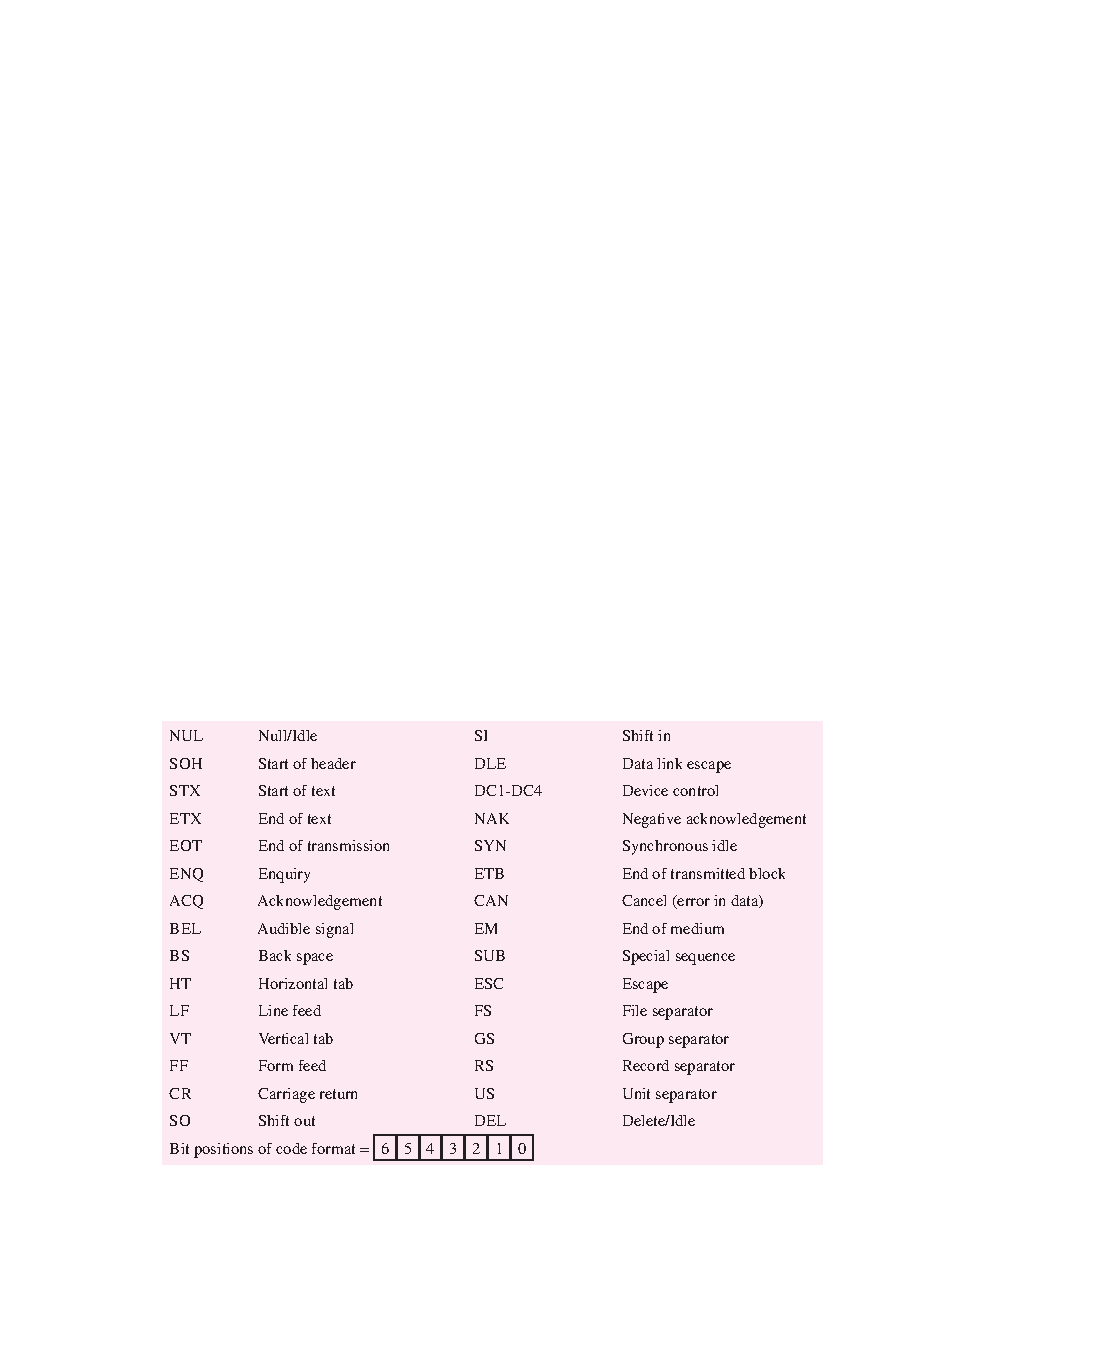
\includegraphics[width=.8\textwidth]{ASCII7S} 
\end{frame}

\begin{frame}{\insertsection}
    \begin{itemize}
        \item O código ASCII usa padrões de sete bits para denotar 128 caracteres diferentes; 
        \item Dez dos caracteres são dígitos decimais de 0 a 9, os bits de alta ordem têm o mesmo padrão, $b_6b_5b_4 = 011$, para todos os 10 dígitos e cada dígito é identificado pelos quatro bits de ordem baixa, $b_{3-0}$, usando os padrões binários para esses dígitos; 
        \item Letras maiúsculas e minúsculas são codificadas de uma maneira que facilita a classificação de informações textuais. Os códigos de A a Z estão em sequência numérica ascendente, o que significa que a tarefa de ordenar letras (ou palavras) pode ser realizada por uma simples comparação aritmética dos códigos que representam as letras;
    \end{itemize}
\end{frame}

\begin{frame}{\insertsection}
    \begin{itemize}
        \item Além de códigos que representam caracteres e letras, o código ASCII inclui sinais de pontuação como \textbf{!} e \textbf{?}, símbolos comumente usados, tais como \textbf{\&} e \textbf{\%} e uma coleção de caracteres de controle;
        \item O padrão ASCII usa sete bits para codificar um caractere.
    \end{itemize}
\end{frame}

\section{Informação Digital e Analógica}

\begin{frame}{\insertsection}
    \centering
    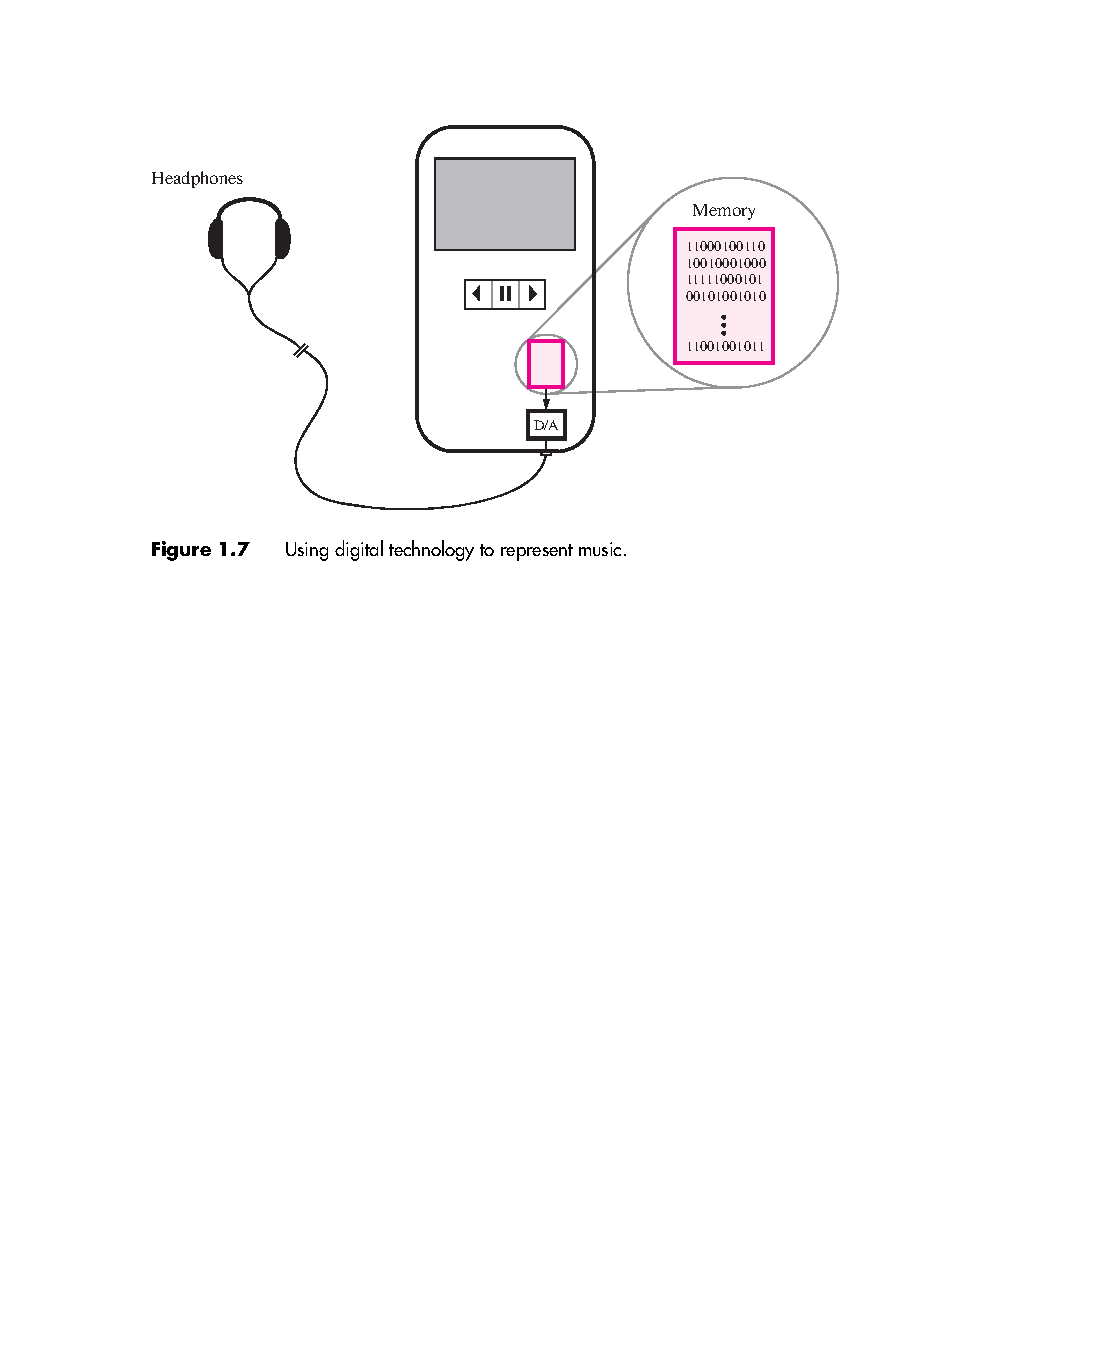
\includegraphics[width=\textwidth]{DigitalAnalog}     
\end{frame}

\section{Teoria e Prática}

\begin{frame}{\insertsection}
    \begin{itemize}
        \item Existem numerosas técnicas para lidar com circuitos lógicos; 
        \item A álgebra booleana, que veremos mais adiante, foi adotada como um meio matemático para representar tais circuitos; 
        \item As ferramentas de CAD\footnote{\textit{computer aided design}} não só tornaram possível projetar circuitos incrivelmente complexos, mas também tornaram o projeto muito mais simples, pois realizam muitas tarefas automaticamente;
    \end{itemize}
\end{frame}

\begin{frame}{\insertsection}
    \begin{itemize}
        \item Por que não aprender simplesmente como usar as ferramentas CAD?
        \begin{itemize}
            \item Elas partem de descrições que, se forem mal especificadas, gerem circuitos de baixa qualidade;
            \item Não é possível compreender o que as ferramentas fazem sem conhecer a teoria subjacente;
            \item Elas oferecem muitas etapas opcionais que devem ou não serem usadas em uma determinada situação;
        \end{itemize}
        \item \textbf{Não é possível tornar-se um projetista de circuitos lógicos efetivo sem entender os conceitos fundamentais!}
    \end{itemize}
\end{frame}


\begin{frame}[fragile]{D'oh!} 
    \begin{columns}
        \begin{column}{0.40\textwidth}
\begin{verbatim}
    ___
   //_\\_
 ."\\    ".
/          \
|           \_
|       ,--.-.)
 \     /  o \o\
 /\/\  \    /_/
  (_.   `--'__)
   |     .-'  \
   |  .-'.     )
   | (  _/--.-'
   |  `.___.'
         (
\end{verbatim}        \end{column}            
        \begin{column}{0.60\textwidth}
            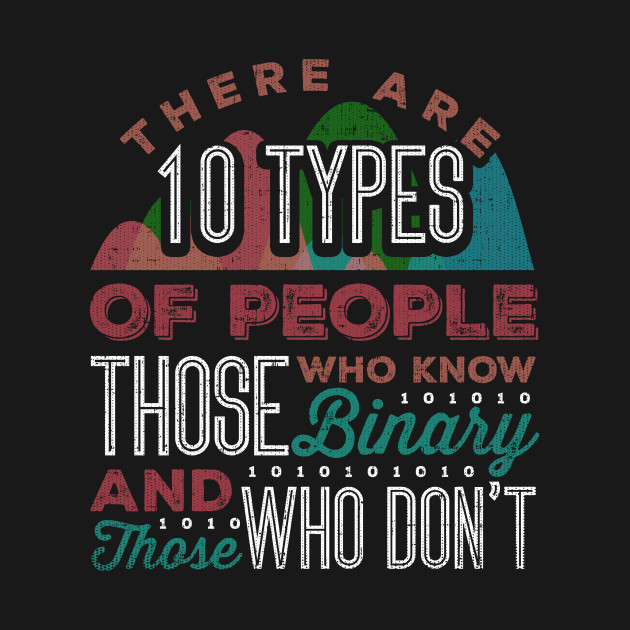
\includegraphics[width=\textwidth]{10people} 
        \end{column}
    \end{columns}
\end{frame}


\section{Bibliografia} %%%%%%%



\begin{frame}{\insertsection} 
	\begin{itemize}
		\item \href{https://www.google.com.br/search?q=filetype\%3Apdf+Fundamentals+of+Digital+Logic+with+Verilog+Design+&oq=filetype\%3Apdf}{Brown, S. \& Vranesic, Z. - Fundamentals of Digital Logic with Verilog Design, 3rd Ed., Mc Graw Hill, 2009}
		\item \href{https://www.asciiart.eu/}{https://www.asciiart.eu/}
	\end{itemize}
\end{frame}


\begin{frame}
	\titlepage
\end{frame} 

\end{document}